\section{Design}
\begin{frame}{Design of the \textit{CORPS}}
\begin{columns}
\column{0.4\textwidth}
    \begin{itemize}
        \item \textit{HIGHYAG BIMO W}
        \item Industrial manipulator
        \item Conveyor
        \item Fixture
        \item Safety measures
    \end{itemize}
\column{0.6\textwidth}
\centering{
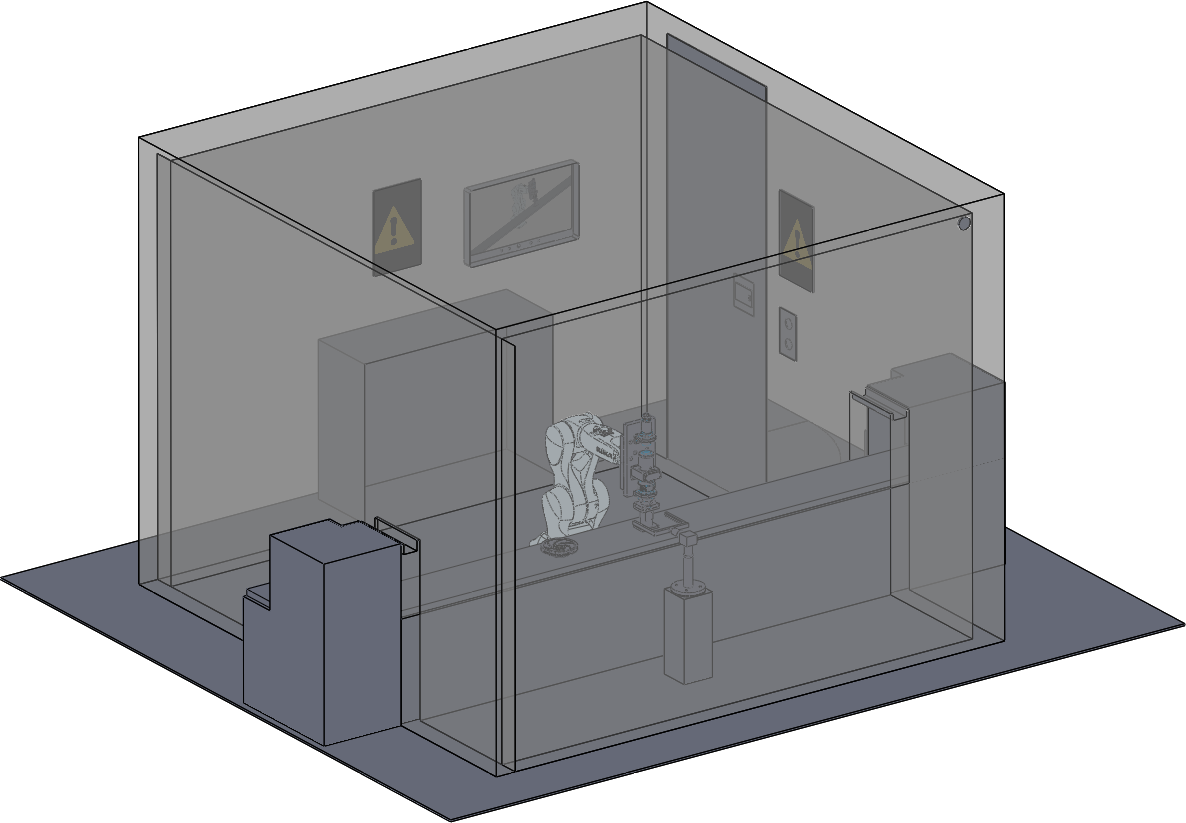
\includegraphics[width=\textwidth]{graphics/andrej/workcell_front_side}}
\end{columns}
\end{frame}




\subsection{Industrial Manipulator}
\begin{frame}{Selection of Industrial Manipulator}{Market Analysis}
\centering{
\includegraphics[width=.975\textwidth]{graphics/andrej/market_analysis}

\tiny{(abb.com) (cloosrobot.com)}}
\end{frame}

\begin{frame}{Selection of Industrial Manipulator}{\textit{KUKA KR 6 R700 sixx}}
\begin{columns}
\column{.53\textwidth}
    \begin{itemize}
        \item \textit{Grundfos}
            \begin{itemize}
                \item Ease the implementation
                \item Reduce the costs
            \end{itemize}
    \vspace{2.5mm}
        \item \textit{KUKA KR 6 R700 sixx}
            \begin{itemize}
                \item Six revolute joints
                \item Maximum payload of $6$ $kg$
                \item Reach of $707$ $mm$
                \item Repeatability of $30\cdot10^{-3}$ $mm$
            \end{itemize}
    \end{itemize}
\column{.47\textwidth}
\centering{
\includegraphics[width=0.775\textwidth]{graphics/andrej/kuka}

\tiny{(kuka.com)}}
\end{columns}
\end{frame}

\subsection{Conveyor System}
\begin{frame}{Selection of Conveyor System}
    \begin{itemize}
        \item Chain conveyor manufactured by \textit{CALDAN CONVEYOR A/S}
            \begin{itemize}
                \item \textit{Grundfos}
            \end{itemize}
    \end{itemize}
\vspace{5mm}
\centering{
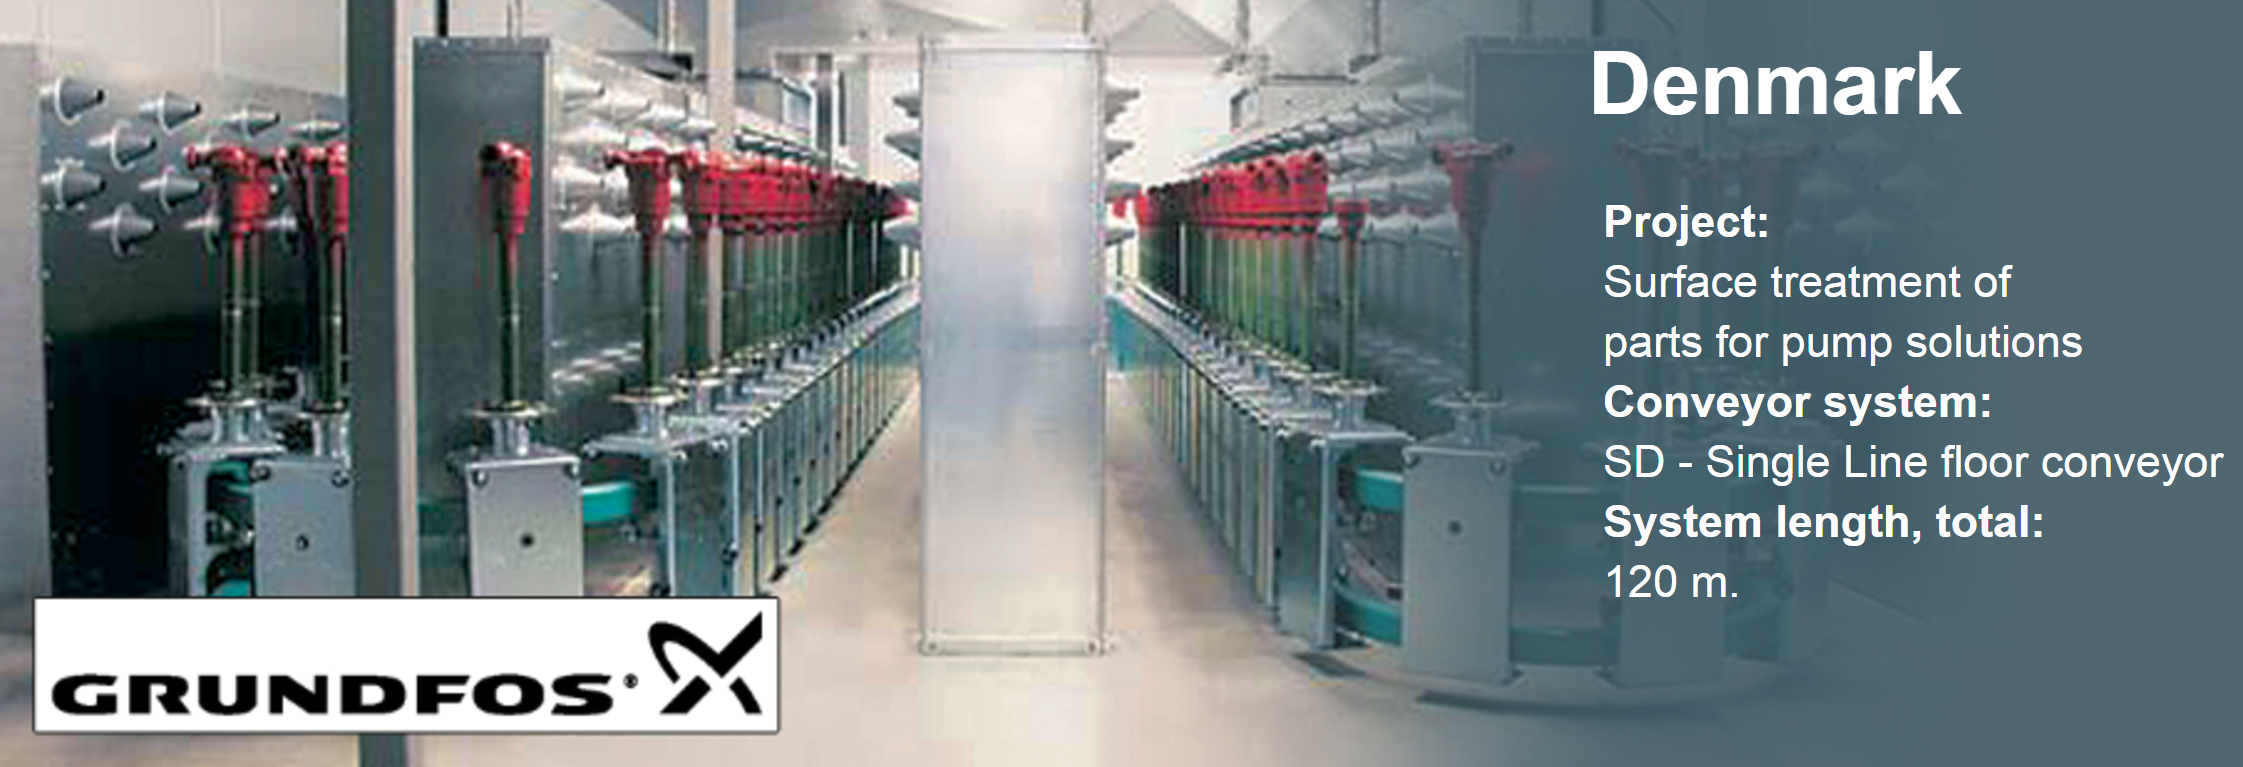
\includegraphics[width=0.9\textwidth]{graphics/andrej/conveyor}

\tiny{(caldan.dk)}}
\end{frame}


\subsection{Fixture}
\begin{frame}{Fixture}{Design Suggestion}
\begin{itemize}
    \item Accessible welding trajectories on both sides
    \item Manually actuated clamps holding the vanes in place
    \item Flippable
\end{itemize}

\begin{columns}
\column{.5\textwidth}
  \centering
  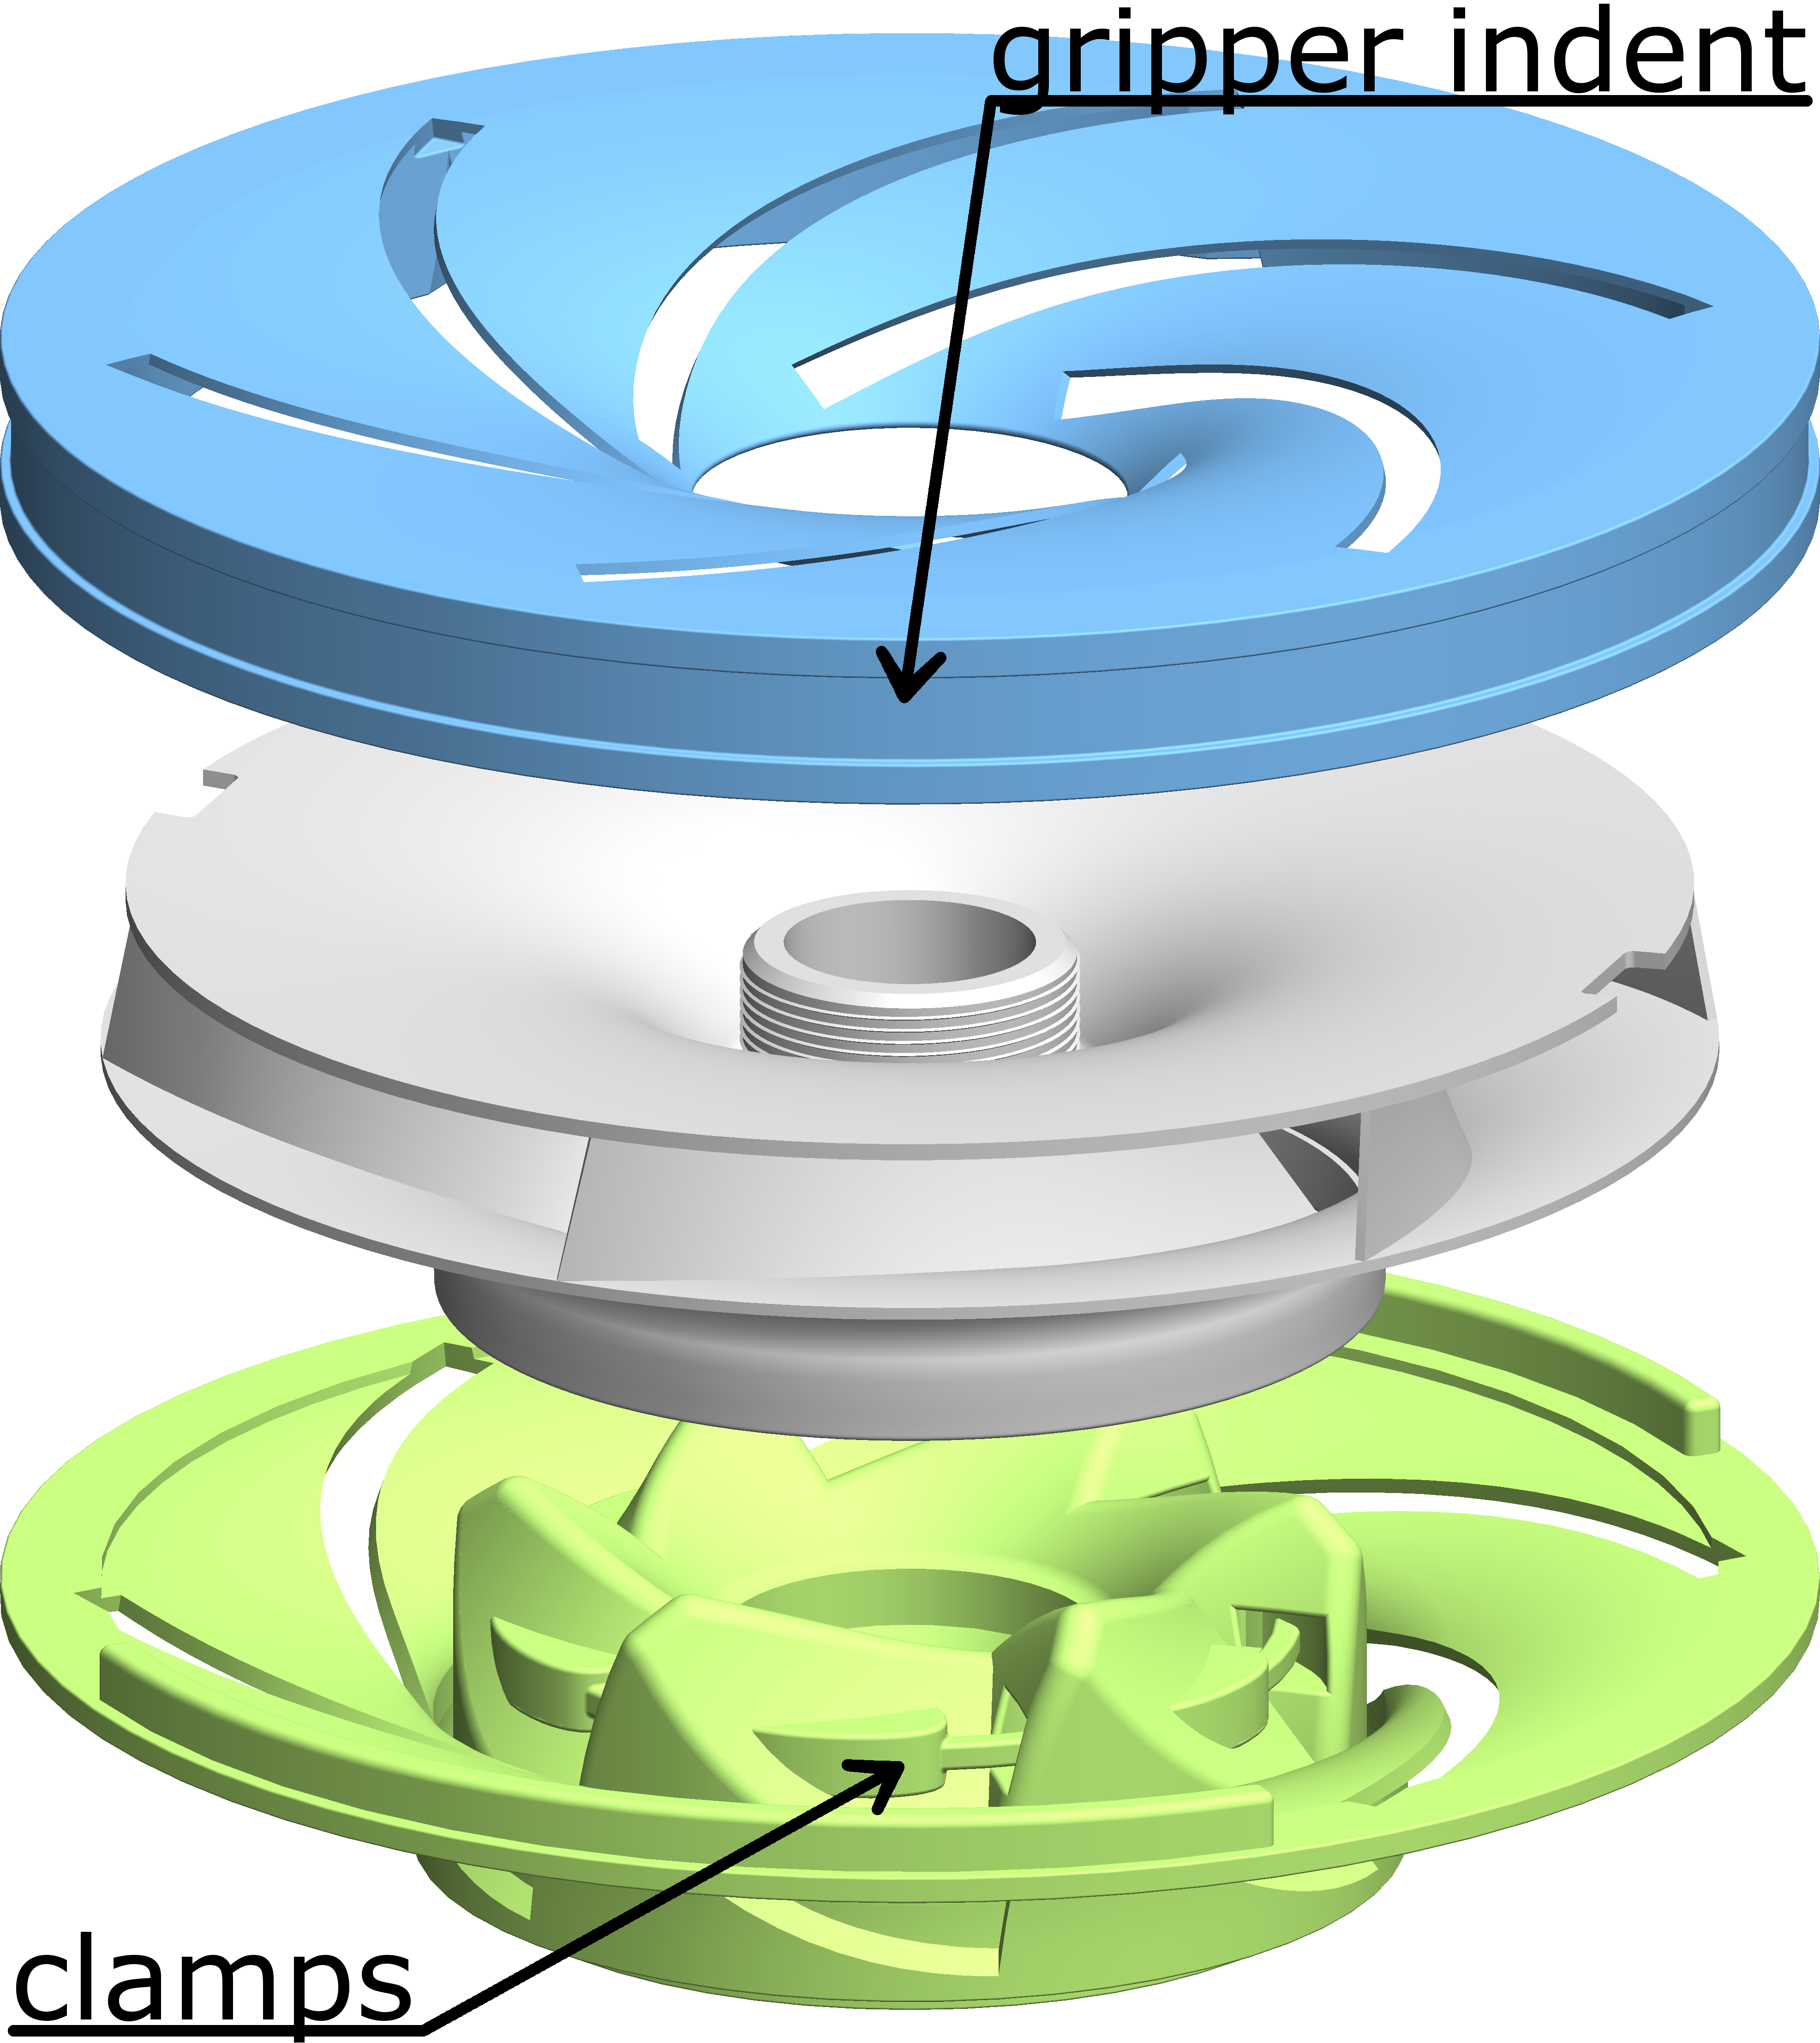
\includegraphics[width=.85\textwidth]{graphics/andrej/if_top}
\column{.5\textwidth}
  \centering
    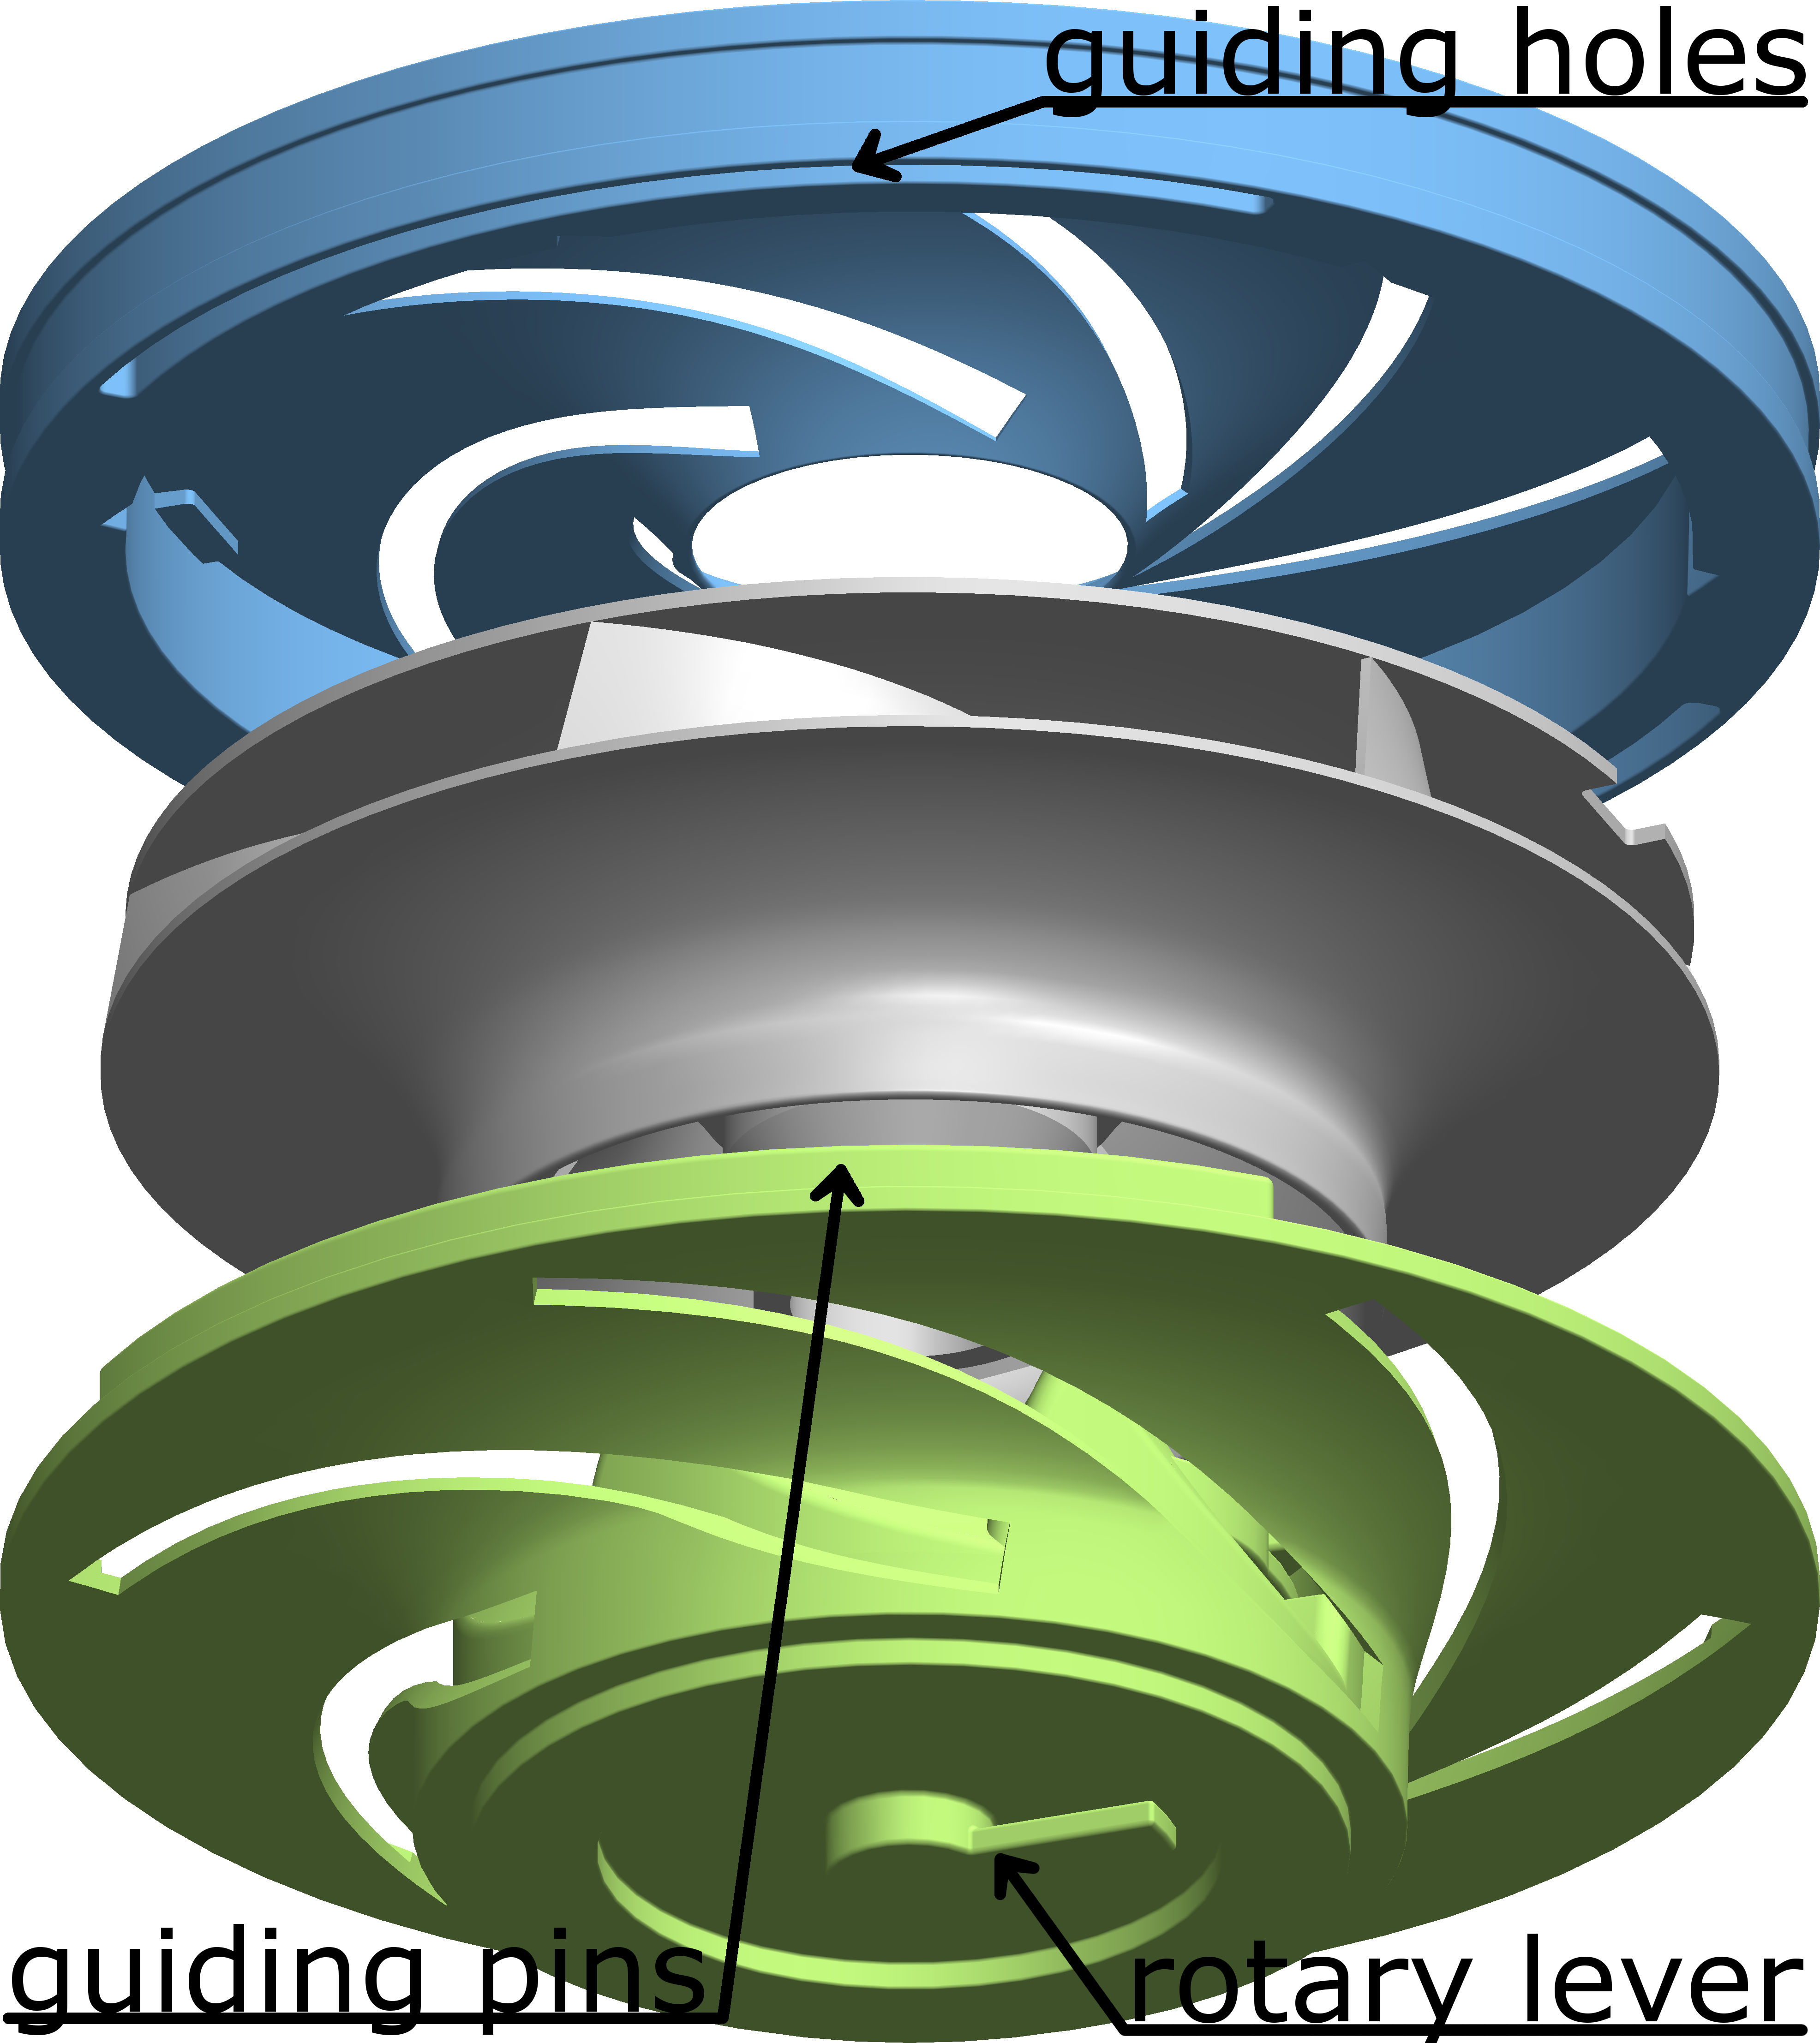
\includegraphics[width=.85\textwidth]{graphics/andrej/if_bottom}
\end{columns}
\end{frame}

\begin{frame}{Fixture}{Fixture Flipping and Fixing System}
 \centering
    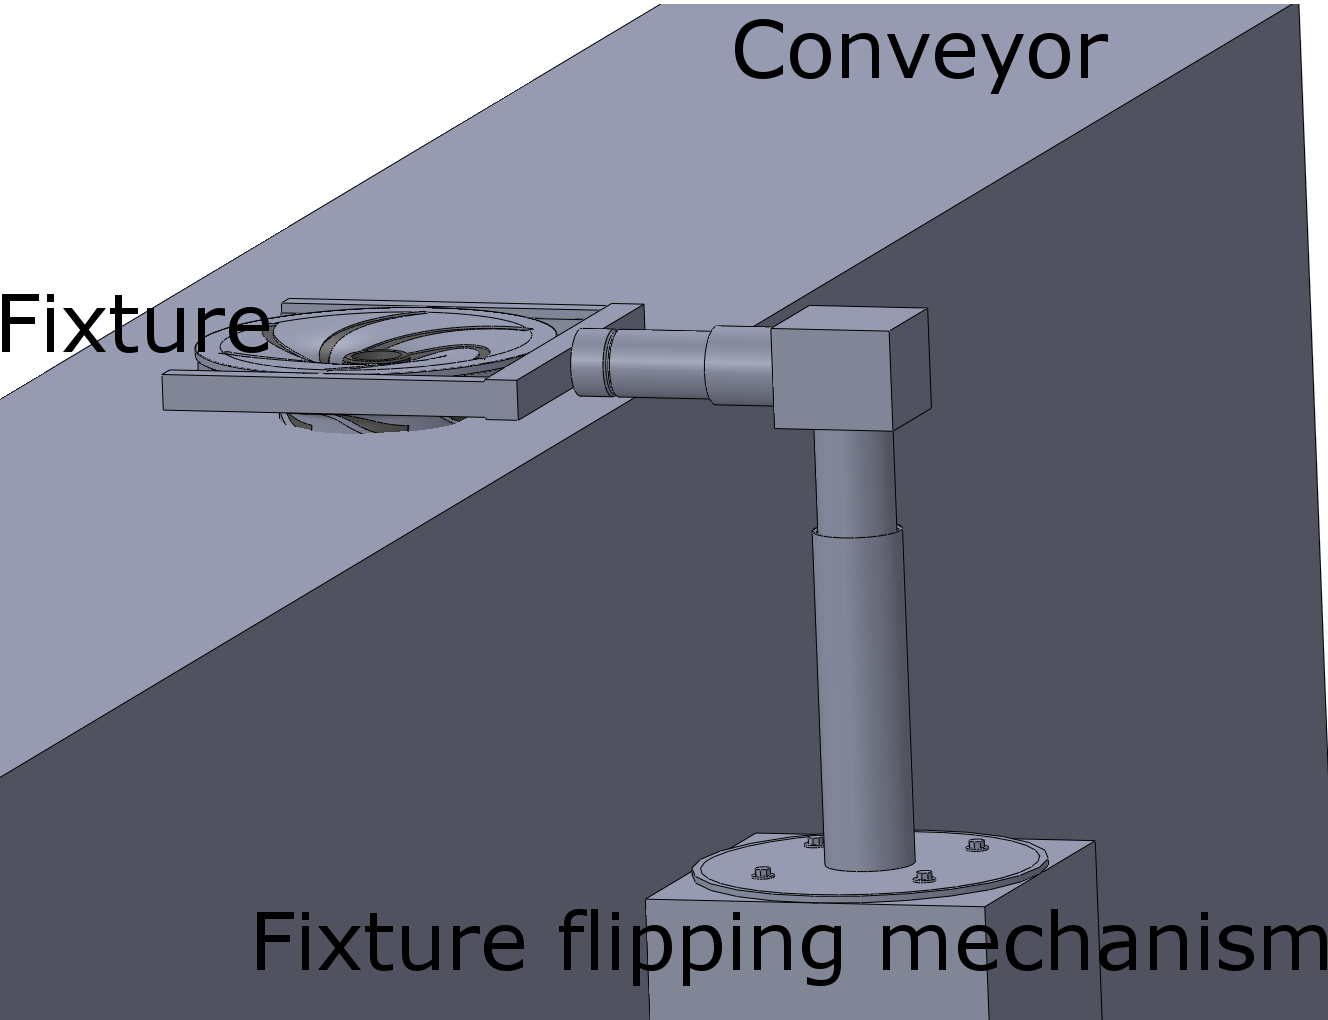
\includegraphics[width=0.9\textwidth]{graphics/andrej/fixture_flipping_mechanism}
\end{frame}















\subsection{Safety Precautions}
\begin{frame}{Risk Assessment}{HUGO}
\begin{itemize}
    \item \textit{ISO 12100}
    \item Origins of hazard
        \begin{itemize}
            \item Laser radiation
            \item Emission of metal fumes
            \item Industrial manipulator
            \item Conveyor 
        \end{itemize}
    \end{itemize}
\end{frame}

\begin{frame}{Risk Reduction}
\begin{itemize}
    \item Guards
        \begin{itemize}
            \item Perimeter wall and ceiling
            \item Laser barriers attached to the wall and ceiling % 10,000W per cm2 with beam site of 5mm for 100 seconds
        \end{itemize}
    \item Ventilation system
    \item Interlocking devices
    \item Material flow monitoring
    \item Welding camera
    \item Emergency button
    \item Informative signs
\end{itemize}
\end{frame}